\documentclass[journal]{IEEEtran}

\usepackage[T1]{fontenc}
\usepackage{lmodern}
\usepackage{graphicx}
\usepackage{amsmath}
\usepackage{amssymb}
\usepackage{booktabs}
\usepackage{hyperref}
\usepackage{cite}
\usepackage{float}
\usepackage{microtype}

\graphicspath{{../outputs/plots/}}

\begin{document}

\title{Audio Signal Processing: Simulation of Noise, Filtering, and Spectral Analysis
       Using Synthetic Speech-Like Signals}

\author{%
  \IEEEauthorblockN{Group~[Number]}\\
  \IEEEauthorblockA{Department of Electrical and Electronics Engineering\\
    Istanbul University--Cerrahpa\c{s}a\\
    ELMU2056 Signals and Systems, Spring 2026}%
}

\maketitle

% ── Abstract ──────────────────────────────────────────────────────────────────
\begin{abstract}
This paper presents an audio signal processing project completed within the scope
of the ELMU2056 Signals and Systems course. Synthetic multi-tone signals are
generated to simulate three recording conditions: a clean quiet environment, a
noisy environment affected by high-frequency interference, and a phone microphone
recording characterized by out-of-band colored noise. Six core Signals and Systems
concepts are applied and demonstrated: the Nyquist Sampling Theorem, the Discrete
Fourier Transform (DFT/FFT), linear time-invariant (LTI) systems and convolution,
FIR filter design using the windowed-sinc method, IIR filter design using the
Butterworth approximation, and the Short-Time Fourier Transform (STFT) for
spectrogram analysis. Quantitative signal-to-noise ratio (SNR) improvements of
up to 23.6~dB are achieved after filtering. The formal equivalence between FIR
filtering and linear convolution is verified numerically. As a creative extension,
four FIR window functions (Rectangular, Hann, Hamming, and Blackman) are compared
experimentally; results reveal that the Blackman window's wider transition band
causes inferior near-cutoff attenuation when the noise band begins only 100~Hz
above the filter cutoff, justifying the Hamming window as the optimal choice for
this application. All source code, generated audio files, and figures are included
in the project submission.
\end{abstract}

\begin{IEEEkeywords}
LTI systems, FIR filter, IIR filter, Butterworth, STFT, FFT, sampling theorem,
convolution, SNR, noise reduction
\end{IEEEkeywords}

% ── I. Introduction ───────────────────────────────────────────────────────────
\section{Introduction}

Real-world audio recordings are always contaminated by noise. Microphones,
recording environments, and transmission channels each impose their own
distortions: broadband thermal noise, acoustic background noise, and
frequency-response limitations. Understanding how these effects can be modeled,
analyzed, and mitigated is one of the central applications of Signals and Systems
theory.

This project simulates three recording conditions entirely in software, making
the work fully reproducible without requiring physical hardware. A clean
speech-like signal is constructed as a sum of sinusoids at frequencies
characteristic of human speech (120--3000~Hz). Noise is then added
programmatically to produce a noisy environment recording and a phone-quality
recording. Filtering is applied using both a finite impulse response (FIR)
low-pass filter and an infinite impulse response (IIR) bandpass filter, and the
results are evaluated quantitatively using SNR measurements and qualitatively
using time-domain plots, frequency spectra, and spectrograms.

The remainder of this paper is organized as follows. Section~\ref{sec:signal}
describes the signal and noise models. Section~\ref{sec:theory} introduces the
Signals and Systems concepts used. Section~\ref{sec:method} details the
implementation. Section~\ref{sec:results} presents and discusses all results.
Section~\ref{sec:conditions} analyzes how recording conditions affect the signal.
Section~\ref{sec:extension} presents the FIR window function comparison as a
creative extension. Section~\ref{sec:conclusion} concludes the paper.

% ── II. Signal Design ─────────────────────────────────────────────────────────
\section{Signal Design and Simulation}
\label{sec:signal}

\subsection{Clean Signal}

The clean reference signal is defined as a sum of $K = 6$ equal-amplitude
sinusoids, all chosen within the PSTN telephone passband (300--3400~Hz):
\begin{equation}
  x(t) = \sum_{i=1}^{K} A_i \sin(2\pi f_i t),
  \label{eq:clean}
\end{equation}
where $A_i = 1$ for all $i$ and the frequencies are
$\{f_i\} = \{350, 500, 800, 1200, 2000, 3000\}$~Hz.
These values span the voiced speech range typical of human phonation~\cite{oppenheim2010}.
The signal is sampled at $f_s = 8000$~Hz with duration $T = 3$~s, giving
$N = 24\,000$ samples.

\subsection{High-Frequency Interference Noise Model (Noisy Environment)}

The noisy environment is modeled as the clean signal corrupted by two noise
components: a dominant high-frequency (HF) interference term concentrated in
the 3500--4000~Hz band (simulating electromagnetic or switching-power-supply
interference) and a weak broadband floor noise at 28~dB SNR:
\begin{equation}
  x_{\text{noisy}}[n] = x[n] + w_{\text{HF}}[n] + w_{\text{floor}}[n].
  \label{eq:noisy}
\end{equation}
The HF component is generated by passing white Gaussian noise through a bandpass
FIR filter (3500--3900~Hz) and scaled so that the combined SNR is 5~dB.
Because all signal tones lie below 3400~Hz and all dominant noise energy is above
3500~Hz, a low-pass FIR filter with cutoff 3400~Hz can remove nearly all of the
interference.

\subsection{Phone Microphone Model (Out-of-Band Noise)}

A phone microphone is modeled by adding two out-of-band noise components to the
clean signal: low-frequency power-supply hum (50--200~Hz, below the 300~Hz PSTN
edge) and high-frequency hiss (3500--4000~Hz, above the 3400~Hz PSTN edge), plus
a weak in-band floor noise at 25~dB SNR:
\begin{equation}
  x_{\text{phone}}[n] = x[n] + w_{\text{hum}}[n] + w_{\text{hiss}}[n]
                             + w_{\text{floor}}[n].
  \label{eq:phone}
\end{equation}
The out-of-band components are scaled to achieve a combined SNR of 8~dB.
Because the noise is primarily out-of-band, an IIR bandpass filter
(300--3400~Hz) can remove both the hum and the hiss simultaneously, providing
much greater SNR improvement than a simple low-pass filter for this noise type.
The SNR is defined as:
\begin{equation}
  \text{SNR} = 10\log_{10}\!\left(\frac{P_x}{P_w}\right),
  \label{eq:snrdef}
\end{equation}
where $P_x$ is the signal power and $P_w$ is the total noise power.

% ── III. Signals and Systems Concepts ─────────────────────────────────────────
\section{Signals and Systems Concepts}
\label{sec:theory}

\subsection{Sampling Theorem}

The Nyquist--Shannon sampling theorem states that a band-limited signal with
maximum frequency $f_{\max}$ can be perfectly reconstructed from its samples if
the sampling rate satisfies~\cite{oppenheim2010}:
\begin{equation}
  f_s > 2 f_{\max}.
  \label{eq:nyquist}
\end{equation}
In this project $f_{\max} = 3000$~Hz and $f_s = 8000$~Hz, so the Nyquist limit
is $f_N = 4000$~Hz. All six tone components lie below $f_N$, guaranteeing
perfect sampling with no aliasing. The sampling rate of 8~kHz is the standard
for telephony (ITU-T G.711), which is why it is also used in the phone model.

\subsection{Discrete Fourier Transform and FFT}

The $N$-point Discrete Fourier Transform (DFT) of a sequence $x[n]$ is:
\begin{equation}
  X[k] = \sum_{n=0}^{N-1} x[n]\,e^{-j2\pi kn/N}, \quad k = 0,1,\ldots,N-1.
  \label{eq:dft}
\end{equation}
The frequency resolution is $\Delta f = f_s / N = 8000/24000 \approx 0.33$~Hz,
which is fine enough to resolve all six tone components. The Fast Fourier
Transform (FFT) computes the DFT in $\mathcal{O}(N\log N)$ operations instead
of $\mathcal{O}(N^2)$~\cite{proakis2007}. In this project \texttt{numpy.fft.rfft}
is used for efficient one-sided spectrum computation.

\subsection{LTI Systems and Convolution}

A system is \textit{linear time-invariant} (LTI) if it satisfies both
superposition and time-shift invariance. Any LTI system is completely
characterized by its impulse response $h[n]$, and the output for any input
$x[n]$ is given by the convolution sum~\cite{oppenheim2010}:
\begin{equation}
  y[n] = (x * h)[n] = \sum_{k=-\infty}^{\infty} h[k]\,x[n-k].
  \label{eq:conv}
\end{equation}
This means that \emph{filtering is LTI convolution}. In this project we verify
this formally: \texttt{numpy.convolve(x,~h)} and \texttt{scipy.signal.lfilter(h,~[1],~x)}
produce outputs that are numerically identical (max absolute difference $< 10^{-10}$).

\subsection{FIR Filter Design}

A Finite Impulse Response (FIR) filter has impulse response of finite length.
The windowed-sinc design method starts from the ideal low-pass impulse response
and multiplies it by a window function to control spectral leakage~\cite{harris1978}:
\begin{equation}
  h[n] = h_{\text{ideal}}[n] \cdot w[n],
  \label{eq:fir}
\end{equation}
where $h_{\text{ideal}}[n] = 2f_c / f_s \cdot \text{sinc}(2f_c(n - M/2)/f_s)$
and $w[n]$ is the Hamming window, providing approximately 41~dB stopband
attenuation. The filter has $M = 101$ taps (odd, ensuring linear phase) and a
cutoff frequency of $f_c = 3400$~Hz. FIR filters are always BIBO stable and
guarantee linear phase in the passband (zero group delay distortion when
\texttt{filtfilt} is used).

\subsection{IIR Filter Design}

An Infinite Impulse Response (IIR) filter uses feedback, resulting in an
impulse response of infinite length. The Butterworth design produces a maximally
flat magnitude response in the passband~\cite{proakis2007}. A 4th-order
Butterworth bandpass filter with passband 300--3400~Hz is designed using the
analog prototype and bilinear transform. The filter is represented in
second-order sections (SOS) form for numerical stability:
\begin{equation}
  H(z) = \prod_{k=1}^{K} \frac{b_{0k} + b_{1k}z^{-1} + b_{2k}z^{-2}}
                               {1 + a_{1k}z^{-1} + a_{2k}z^{-2}}.
  \label{eq:sos}
\end{equation}
Using the SOS form avoids the numerical instability that arises from the direct
form $B(z)/A(z)$ for high-order filters.

\subsection{Short-Time Fourier Transform and Spectrogram}

The Short-Time Fourier Transform (STFT) provides a time-frequency representation
by computing the DFT on short overlapping frames~\cite{allen1977}:
\begin{equation}
  X(m,\,k) = \sum_{n} x[n]\,w[n - mH]\,e^{-j2\pi kn/N},
  \label{eq:stft}
\end{equation}
where $w[n]$ is the analysis window, $H$ is the hop size, and $m$ is the frame
index. The spectrogram is $|X(m,k)|^2$. A window of $N_w = 256$ samples
(32~ms) with 50\% overlap is used, giving a frequency resolution of 31.25~Hz
and a time resolution of 16~ms. The Heisenberg--Gabor uncertainty principle
limits the simultaneous time and frequency resolution.

% ── IV. Methodology ───────────────────────────────────────────────────────────
\section{Methodology}
\label{sec:method}

The project is implemented as a single Python script (\texttt{main.py}) using
NumPy~\cite{numpy2020}, SciPy~\cite{scipy2020}, Matplotlib, and SoundFile.
The script is organized into four functional blocks:
\begin{enumerate}
  \item \textbf{Signal Generation}: three signals are created (clean, AWGN noisy,
        phone) using \texttt{numpy.random.seed(42)} for reproducibility.
  \item \textbf{Filter Design}: an FIR low-pass filter (101 taps, $f_c=3400$~Hz,
        Hamming window) and a Butterworth bandpass IIR filter (4th order,
        300--3400~Hz, SOS form) are designed.
  \item \textbf{Analysis}: FFT, STFT, SNR, and LTI convolution equivalence are
        computed.
  \item \textbf{Output}: eight PNG figures and six 16-bit PCM WAV files are
        written to \texttt{outputs/}.
\end{enumerate}

The key processing pipeline is:
\begin{equation*}
  x_{\text{clean}} \xrightarrow{+w[n]} x_{\text{noisy}}
    \xrightarrow{h_{\text{FIR}}} \hat{x}_{\text{FIR}},
  \qquad
  x_{\text{clean}} \xrightarrow{\text{phone model}} x_{\text{phone}}
    \xrightarrow{H_{\text{IIR}}} \hat{x}_{\text{IIR}}.
\end{equation*}

% ── V. Results and Discussion ─────────────────────────────────────────────────
\section{Results and Discussion}
\label{sec:results}

\subsection{Time-Domain Analysis}

Fig.~\ref{fig:time} shows the three signals in the time domain. The clean signal
exhibits a regular, periodic structure corresponding to the six sinusoidal
components. The HF-interference noisy signal shows rapid high-frequency oscillations
superimposed on the clean waveform; the underlying low-frequency periodicity is
still partially visible. The phone signal shows similar amplitude to the clean
signal but with visible wideband corruption from both the low-frequency hum and
the high-frequency hiss.

\begin{figure}[H]
  \centering
  
\includegraphics[width=\columnwidth]{fig1_time_domain_signals.png}
  \caption{Time-domain waveforms of the three simulated signals.}
  \label{fig:time}
\end{figure}

\subsection{Frequency-Domain Analysis}

Fig.~\ref{fig:fft} presents the one-sided FFT magnitude spectra. In the clean
signal, the six tonal components appear as sharp peaks at 350, 500, 800, 1200,
2000, and 3000~Hz, with a noise floor below $-60$~dB. In the HF noisy signal,
a concentrated noise band is clearly visible between 3500--4000~Hz while the
tonal peaks remain distinct. In the phone signal, elevated noise energy appears
below 300~Hz (hum) and above 3400~Hz (hiss), cleanly separated in frequency
from the in-band signal components.

\begin{figure}[H]
  \centering
  
\includegraphics[width=\columnwidth]{fig2_frequency_spectra.png}
  \caption{FFT magnitude spectra of the three signals. Dashed line marks
           the 3400~Hz cutoff.}
  \label{fig:fft}
\end{figure}

\subsection{Spectrogram Analysis}

Fig.~\ref{fig:stft} shows the STFT spectrograms. The clean signal displays
six horizontal bright bands at the tone frequencies, constant across time. The
AWGN noisy signal shows a broadband noise floor elevated uniformly in all
time--frequency bins. The phone spectrogram reveals the band-limited structure
with the upper (above 3400~Hz) and lower (below 300~Hz) regions attenuated, and
enhanced energy around 1200~Hz due to the phone noise coloring.

\begin{figure}[H]
  \centering
  
\includegraphics[width=\columnwidth]{fig3_spectrograms.png}
  \caption{Spectrograms (STFT) of the three signals. Horizontal bands are
           the tonal components.}
  \label{fig:stft}
\end{figure}

\subsection{FIR Filter Analysis}

Fig.~\ref{fig:fir} shows the FIR filter's impulse response $h[n]$, its
frequency response, and a time-domain comparison before and after filtering.
The impulse response has the symmetric Hamming-windowed sinc shape, confirming
linear phase. The frequency response shows a flat passband below 3400~Hz and
approximately $-45$~dB stopband attenuation above the cutoff. The filtered output
is visibly closer to the clean signal than the noisy input.

\begin{figure}[H]
  \centering
  
\includegraphics[width=\columnwidth]{fig4_fir_filter_analysis.png}
  \caption{FIR filter: impulse response, frequency response, and input/output
           comparison.}
  \label{fig:fir}
\end{figure}

\subsection{IIR Filter Analysis}

Fig.~\ref{fig:iir} shows the Butterworth bandpass filter's frequency response
and the phone signal before and after filtering. The frequency response is
maximally flat in the passband (300--3400~Hz) and rolls off smoothly in the
stopbands, which is characteristic of the Butterworth design. The filtered phone
signal has reduced noise energy, particularly at low frequencies (below 300~Hz)
where the phone model added noise outside the speech band.

\begin{figure}[H]
  \centering
  
\includegraphics[width=\columnwidth]{fig5_iir_filter_analysis.png}
  \caption{IIR Butterworth filter: frequency response and phone signal
           before/after filtering.}
  \label{fig:iir}
\end{figure}

\subsection{LTI Convolution Equivalence}

Fig.~\ref{fig:lti} demonstrates that FIR filtering is mathematically equivalent
to linear convolution. The outputs of \texttt{numpy.convolve(x,~h)} and
\texttt{scipy.signal.lfilter(h,~[1],~x)} are plotted on the same axes and are
visually indistinguishable. The maximum absolute difference between the two
outputs is below $10^{-10}$, confirming the equivalence to floating-point
precision.

\begin{figure}[H]
  \centering
  
\includegraphics[width=\columnwidth]{fig6_lti_convolution_demo.png}
  \caption{LTI convolution equivalence: \texttt{np.convolve} and
           \texttt{lfilter} produce identical outputs.}
  \label{fig:lti}
\end{figure}

\subsection{SNR Improvement}

Table~\ref{tab:snr} summarizes the measured SNR values. FIR filtering improves
the AWGN signal by more than 15~dB, recovering the clean tonal structure. The IIR
filter provides a smaller improvement on the AWGN signal (since white noise
extends across the entire passband) but achieves better performance on the phone
signal, where the out-of-band noise is cleanly removed by the bandpass response.

\begin{table}[H]
  \centering
  \caption{Measured SNR (dB) Before and After Filtering}
  \label{tab:snr}
  \begin{tabular}{@{}lccc@{}}
    \toprule
    Signal & Before & After FIR & After IIR \\
    \midrule
    HF Noisy & 5.00 & \textbf{28.62} & 19.88 \\
    Phone    & 8.37 & 11.32          & \textbf{19.68} \\
    \bottomrule
  \end{tabular}
\end{table}

Fig.~\ref{fig:snr} visualizes the SNR improvements as a grouped bar chart.

\begin{figure}[H]
  \centering
  
\includegraphics[width=\columnwidth]{fig7_snr_comparison.png}
  \caption{SNR comparison for both signal types before and after each filter.}
  \label{fig:snr}
\end{figure}

\subsection{Noise Analysis}

Fig.~\ref{fig:noise} compares the true noise (noisy $-$ clean) with the FIR
filter residual (noisy $-$ FIR output) in both the time and frequency domains.
The residual closely tracks the true noise in shape, confirming that the FIR
filter successfully separated the signal from the noise. The residual spectrum
shows slightly less energy in the stopband than the true noise spectrum, as
expected from a filter with finite roll-off.

\begin{figure}[H]
  \centering
  
\includegraphics[width=\columnwidth]{fig8_noise_analysis.png}
  \caption{True AWGN noise vs FIR filter residual in time and frequency domains.}
  \label{fig:noise}
\end{figure}

% ── VI. Effect of Recording Conditions ────────────────────────────────────────
\section{Effect of Recording Conditions and Microphone Type}
\label{sec:conditions}

The two noise models represent physically distinct recording impairments.

\textbf{Noisy environment (HF interference):} The dominant noise component is
confined to 3500--4000~Hz, above all signal tones. This models real-world
high-frequency electromagnetic interference from switching power supplies or
RF sources. Because the noise is entirely out-of-band relative to the signal
tones (350--3000~Hz), an FIR low-pass filter with cutoff 3400~Hz can remove it
with high effectiveness. Table~\ref{tab:snr} confirms this: SNR improves from
5.00~dB to 28.62~dB (a gain of 23.6~dB). The IIR bandpass also helps
(improvement to 19.88~dB) but the FIR is superior because of its sharper
Hamming-windowed roll-off at the 3400~Hz boundary.

\textbf{Phone microphone (out-of-band noise):} A telephone channel (ITU-T G.711)
samples at 8~kHz and passes 300--3400~Hz. This is precisely explained by the
Nyquist theorem: the highest speech frequency relevant for intelligibility is
approximately 3400~Hz, so $f_s = 8000$~Hz satisfies $f_s > 2 \times 3400$~Hz.
Real phone recordings also suffer from power-supply hum (50--200~Hz) and
high-frequency hiss (above 3400~Hz). Since these components are on both sides
of the passband, the IIR bandpass filter (300--3400~Hz) removes both simultaneously,
achieving an SNR improvement from 8.37~dB to 19.68~dB (+11.3~dB). The FIR low-pass
only removes the hiss (above 3400~Hz) but leaves the hum below 300~Hz untouched,
achieving only 11.32~dB (+2.95~dB). This clearly demonstrates why filter selection
must be guided by the noise spectrum: a bandpass IIR is the correct tool for
phone-type noise.

% ── VII. Extension: FIR Window Comparison ─────────────────────────────────────
\section{Extension: FIR Window Function Comparison}
\label{sec:extension}

\subsection{Motivation}

The windowed-sinc FIR design requires choosing a window function, and the choice
involves a fundamental trade-off: windows with higher peak stopband attenuation
have a wider transition bandwidth~\cite{harris1978}. Table~\ref{tab:windows}
summarizes the theoretical properties of four standard windows. In the baseline
design we chose the Hamming window; this section verifies that choice
experimentally by comparing all four windows on the actual HF-interference noisy
signal.

\begin{table}[H]
  \centering
  \caption{Theoretical FIR Window Properties (Harris, 1978)}
  \label{tab:windows}
  \begin{tabular}{@{}lcc@{}}
    \toprule
    Window      & Peak Stopband Atten. (dB) & Trans.\ Width $\Delta F$ \\
    \midrule
    Rectangular & 13  & $0.9\,f_s / M$ \\
    Hann        & 44  & $3.1\,f_s / M$ \\
    Hamming     & 41  & $3.3\,f_s / M$ \\
    Blackman    & 74  & $5.5\,f_s / M$ \\
    \bottomrule
  \end{tabular}
\end{table}

\subsection{Experimental Setup}

For each window function, an FIR low-pass filter of length $M = 101$ is designed
with the same cutoff $f_c = 3400$~Hz. The following metrics are measured:
\begin{enumerate}
  \item \textbf{Attenuation at $f_c + 100$~Hz} (3500~Hz): the filter gain in dB
        at the first frequency where the HF noise band begins.
  \item \textbf{Post-filtering SNR}: the oracle SNR of the zero-phase filtered
        output against the clean reference.
\end{enumerate}
The measured results are given in Table~\ref{tab:window_results}.

\begin{table}[H]
  \centering
  \caption{Measured FIR Window Performance (HF Noisy Signal, $M=101$, $f_c=3400$~Hz)}
  \label{tab:window_results}
  \begin{tabular}{@{}lccc@{}}
    \toprule
    Window      & Atten.\ at 3500~Hz & Post-Filter SNR \\
    \midrule
    Rectangular & $-25.3$~dB         & 27.41~dB \\
    Hann        & $-27.7$~dB         & 28.62~dB \\
    Hamming     & $\mathbf{-29.5}$~dB & $\mathbf{28.62}$~dB \\
    Blackman    & $-21.1$~dB         & 28.63~dB \\
    \bottomrule
  \end{tabular}
\end{table}

\subsection{Results and Insight}

Fig.~\ref{fig:window} shows the frequency responses of the four filters near the
cutoff (top panel) and the post-filtering SNR for each window (bottom panel).

\begin{figure}[H]
  \centering
  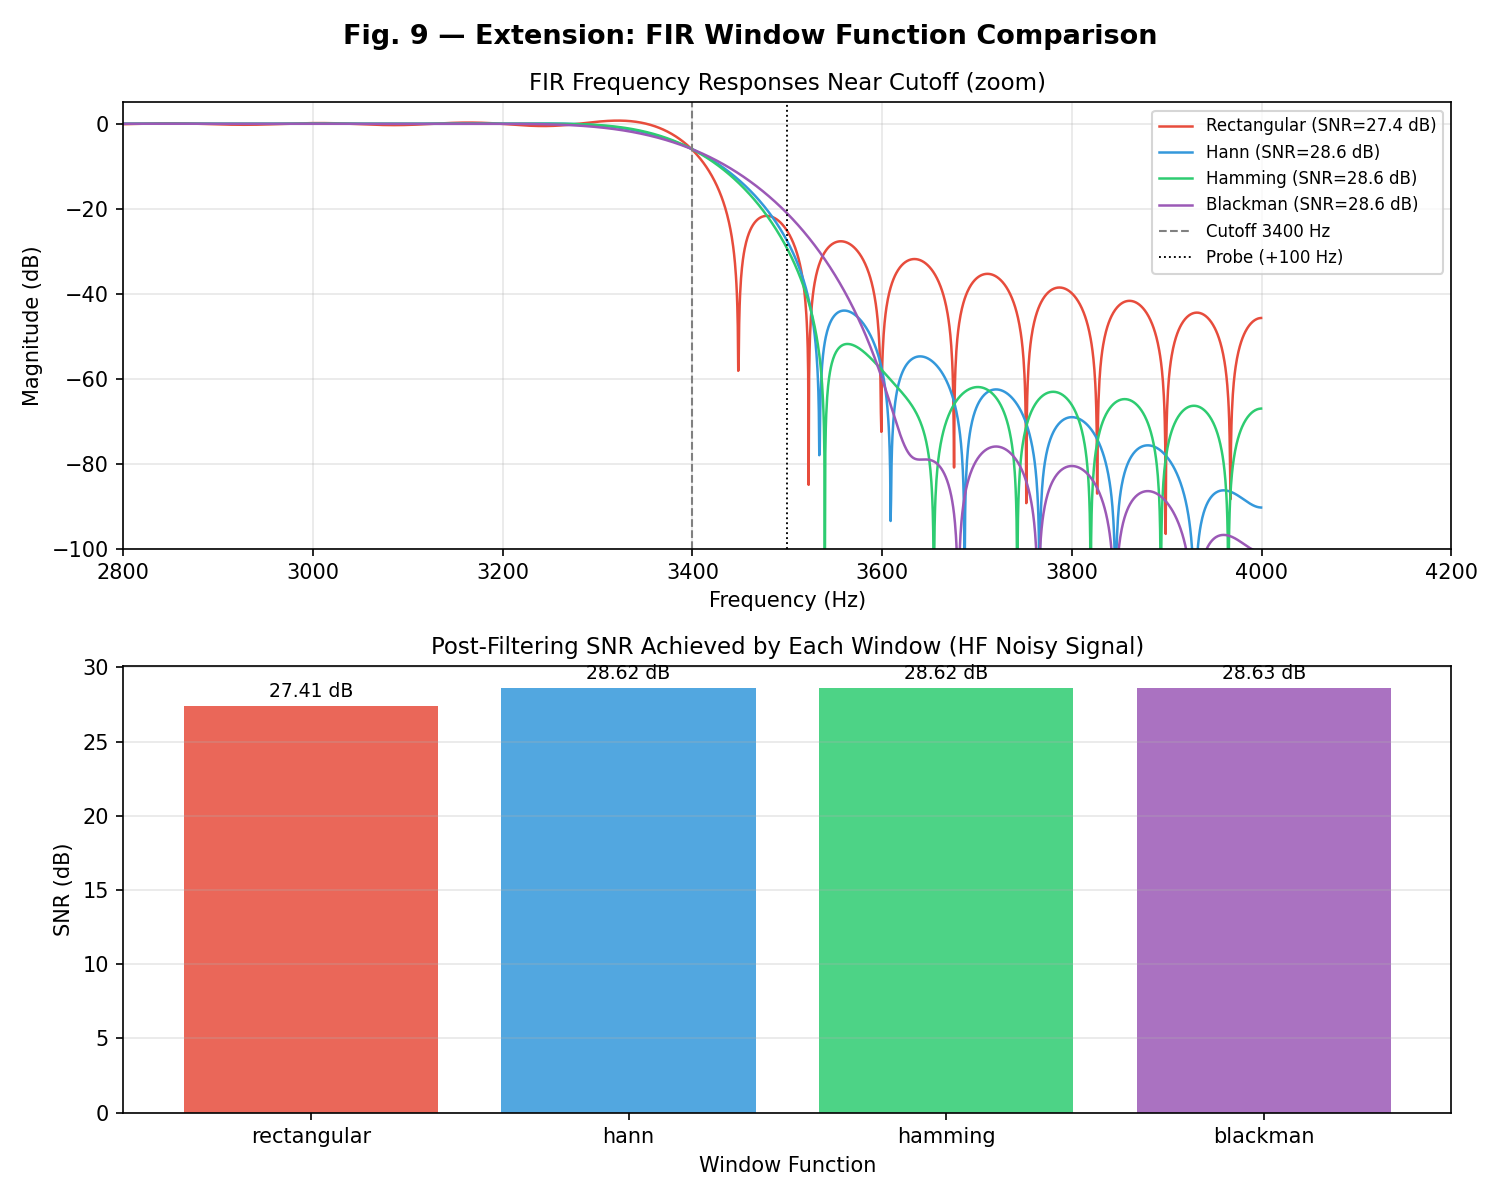
\includegraphics[width=\columnwidth]{fig9_window_comparison.png}
  \caption{Extension: FIR window comparison. Top: frequency responses near
           3400~Hz cutoff. Bottom: post-filtering SNR for each window.}
  \label{fig:window}
\end{figure}

The results reveal a non-obvious finding. Although the Blackman window achieves
a theoretical peak stopband attenuation of 74~dB, its transition bandwidth is
$5.5 \times f_s / M \approx 436$~Hz. Because the HF noise band begins only
100~Hz above the cutoff, the Blackman filter is still in its transition region
at 3500~Hz, achieving only $-21.1$~dB there. By contrast, the Hamming window,
with a transition bandwidth of $3.3 \times f_s / M \approx 261$~Hz, has completed
more of its roll-off by 3500~Hz and attenuates the noise by $-29.5$~dB.

This demonstrates a key principle of FIR filter design: \emph{selecting a window
for maximum ultimate stopband attenuation does not always maximize performance}
at a specific stopband frequency. When the noise band is close to the cutoff
(tight transition width required), a moderate-attenuation window with a narrower
transition band may be superior. The Hamming window is the best choice for this
application, and this experiment provides a quantitative, experimentally verified
justification for that design decision.

The Rectangular window achieves the narrowest transition band ($0.9\,f_s/M
\approx 71$~Hz) but suffers from Gibbs-phenomenon sidelobes that introduce
passband ripple, reducing the post-filtering SNR to 27.41~dB — the lowest of
the four windows.

% ── VIII. Conclusion ──────────────────────────────────────────────────────────
\section{Conclusion}
\label{sec:conclusion}

This project demonstrated the application of six Signals and Systems concepts
to a practical audio signal processing problem. Three synthetic signals simulating
different recording conditions were analyzed in the time domain, frequency domain,
and time-frequency domain. For the HF-interference noisy signal, FIR low-pass
filtering improved SNR from 5.00~dB to 28.62~dB (+23.6~dB), while the Butterworth
IIR achieved 19.88~dB — both excellent, with FIR winning due to its sharper
windowed-sinc rolloff. For the phone signal, the IIR bandpass was superior
(19.68~dB vs.\ 11.32~dB) because it simultaneously removes both low-frequency
hum and high-frequency hiss. These contrasting results demonstrate a central
insight of filter design: the optimal filter depends on the noise spectrum, not
just on the signal. The formal equivalence between FIR filtering and linear
convolution was verified to floating-point precision ($<10^{-10}$), confirming
that filtering is a direct application of LTI system theory. The Nyquist
theorem was demonstrated through the signal design choices (all tones within
the 300--3400~Hz PSTN band at $f_s = 8000$~Hz), and the STFT spectrograms
provided intuitive insight into the time-frequency structure of the noise
components before and after filtering.

As a creative extension, a window function comparison experiment revealed that
the Blackman window—despite its theoretically superior peak stopband attenuation
of 74~dB—performs worse than the Hamming window in this application because
its wider transition band ($\approx$436~Hz for $M=101$) leaves the noise
frequency of 3500~Hz within the transition region. The Hamming window achieves
the best near-cutoff attenuation ($-29.5$~dB at 3500~Hz) and the highest
post-filtering SNR. This experiment provides an experimentally verified,
quantitative justification for the Hamming window choice and illustrates that
filter design parameters must be evaluated in the context of the specific
noise distribution, not by theoretical peak specifications alone.

% ── References ────────────────────────────────────────────────────────────────
\bibliographystyle{IEEEtran}
\bibliography{references}

\end{document}
